\documentclass[journal,12pt,twocolumn]{IEEEtran}
\usepackage{float}
\usepackage{setspace}
\usepackage{gensymb}

\singlespacing


\usepackage[cmex10]{amsmath}

\usepackage{amsthm}

\usepackage{mathrsfs}
\usepackage{txfonts}
\usepackage{stfloats}
\usepackage{bm}
\usepackage{cite}
\usepackage{cases}
\usepackage{subfig}

\usepackage{longtable}
\usepackage{multirow}

\usepackage{enumitem}
\usepackage{mathtools}
\usepackage{steinmetz}
\usepackage{tikz}
\usepackage{circuitikz}
\usepackage{verbatim}
\usepackage{tfrupee}
\usepackage[breaklinks=true]{hyperref}
\usepackage{graphicx}
\usepackage{tkz-euclide}

\usetikzlibrary{calc,math}
\usepackage{listings}
    \usepackage{color}                                            %%
    \usepackage{array}                                            %%
    \usepackage{longtable}                                        %%
    \usepackage{calc}                                             %%
    \usepackage{multirow}                                         %%
    \usepackage{hhline}                                           %%
    \usepackage{ifthen}                                           %%
    \usepackage{lscape}     
\usepackage{multicol}
\usepackage{chngcntr}

\DeclareMathOperator*{\Res}{Res}

\renewcommand\thesection{\arabic{section}}
\renewcommand\thesubsection{\thesection.\arabic{subsection}}
\renewcommand\thesubsubsection{\thesubsection.\arabic{subsubsection}}

\renewcommand\thesectiondis{\arabic{section}}
\renewcommand\thesubsectiondis{\thesectiondis.\arabic{subsection}}
\renewcommand\thesubsubsectiondis{\thesubsectiondis.\arabic{subsubsection}}


\hyphenation{op-tical net-works semi-conduc-tor}
\def\inputGnumericTable{}                                 %%

\lstset{
%language=C,
frame=single, 
breaklines=true,
columns=fullflexible
}
\begin{document}


\newtheorem{theorem}{Theorem}[section]
\newtheorem{problem}{Problem}
\newtheorem{proposition}{Proposition}[section]
\newtheorem{lemma}{Lemma}[section]
\newtheorem{corollary}[theorem]{Corollary}
\newtheorem{example}{Example}[section]
\newtheorem{definition}[problem]{Definition}

\newcommand{\BEQA}{\begin{eqnarray}}
\newcommand{\EEQA}{\end{eqnarray}}
\newcommand{\define}{\stackrel{\triangle}{=}}
\bibliographystyle{IEEEtran}
\providecommand{\mbf}{\mathbf}
\providecommand{\pr}[1]{\ensuremath{\Pr\left(#1\right)}}
\providecommand{\qfunc}[1]{\ensuremath{Q\left(#1\right)}}
\providecommand{\sbrak}[1]{\ensuremath{{}\left[#1\right]}}
\providecommand{\lsbrak}[1]{\ensuremath{{}\left[#1\right.}}
\providecommand{\rsbrak}[1]{\ensuremath{{}\left.#1\right]}}
\providecommand{\brak}[1]{\ensuremath{\left(#1\right)}}
\providecommand{\lbrak}[1]{\ensuremath{\left(#1\right.}}
\providecommand{\rbrak}[1]{\ensuremath{\left.#1\right)}}
\providecommand{\cbrak}[1]{\ensuremath{\left\{#1\right\}}}
\providecommand{\lcbrak}[1]{\ensuremath{\left\{#1\right.}}
\providecommand{\rcbrak}[1]{\ensuremath{\left.#1\right\}}}
\theoremstyle{remark}
\newtheorem{rem}{Remark}
\newcommand{\sgn}{\mathop{\mathrm{sgn}}}
\providecommand{\abs}[1]{\left\vert#1\right\vert}
\providecommand{\res}[1]{\Res\displaylimits_{#1}} 
\providecommand{\norm}[1]{\left\lVert#1\right\rVert}
%\providecommand{\norm}[1]{\lVert#1\rVert}
\providecommand{\mtx}[1]{\mathbf{#1}}
\providecommand{\mean}[1]{E\left[ #1 \right]}
\providecommand{\fourier}{\overset{\mathcal{F}}{ \rightleftharpoons}}
%\providecommand{\hilbert}{\overset{\mathcal{H}}{ \rightleftharpoons}}
\providecommand{\system}{\overset{\mathcal{H}}{ \longleftrightarrow}}
	%\newcommand{\solution}[2]{\textbf{Solution:}{#1}}
\newcommand{\solution}{\noindent \textbf{Solution: }}
\newcommand{\cosec}{\,\text{cosec}\,}
\providecommand{\dec}[2]{\ensuremath{\overset{#1}{\underset{#2}{\gtrless}}}}
\newcommand{\myvec}[1]{\ensuremath{\begin{pmatrix}#1\end{pmatrix}}}
\newcommand{\mydet}[1]{\ensuremath{\begin{vmatrix}#1\end{vmatrix}}}
\numberwithin{equation}{subsection}
\makeatletter
\@addtoreset{figure}{problem}
\makeatother
\let\StandardTheFigure\thefigure
\let\vec\mathbf
\renewcommand{\thefigure}{\theproblem}
\def\putbox#1#2#3{\makebox[0in][l]{\makebox[#1][l]{}\raisebox{\baselineskip}[0in][0in]{\raisebox{#2}[0in][0in]{#3}}}}
     \def\rightbox#1{\makebox[0in][r]{#1}}
     \def\centbox#1{\makebox[0in]{#1}}
     \def\topbox#1{\raisebox{-\baselineskip}[0in][0in]{#1}}
     \def\midbox#1{\raisebox{-0.5\baselineskip}[0in][0in]{#1}}
\vspace{3cm}
\title{Assignment 1}
\author{A.Tejasri}
\maketitle
\newpage
\bigskip
\renewcommand{\thefigure}{\theenumi}
\renewcommand{\thetable}{\theenumi}
Download all python codes from 
\begin{lstlisting}

https://github.com/teja3657/Assignment1/tree/master/CODES
\end{lstlisting}
%
and latex-tikz codes from 
%
\begin{lstlisting}
https://github.com/teja3657/Assignment1/blob/master/Assignment1.tex
\end{lstlisting}
%
\section{Question No.2.16}
Construct an isosceles triangle in which the lengths of the equal sides is 6.5 and the angle between them is $110{\degree}$.
%
\section{SOLUTION}
The vertices are:
\begin{align}
\vec{L} = \myvec{0\\0},
\vec{D} = \myvec{ld\\0}, 
\vec{O} = \myvec{p1\\q1}
\end{align}
Finding $\angle O$ and $\angle D$:

In $\triangle OLD$,
\begin{align}
\angle O+\angle L+\angle D&=180^{\degree}
\quad\brak{\because \angle O=\angle D=x}
\\
\ x+110^{\degree}+x&=180^{\degree}
\\
\ 2x &=180^{\degree}-110^{\degree}
\\
\ 2x &=70^{\degree}
\\
\ x &=35^{\degree} \quad\brak{\because \angle O=\angle D=35^{\degree}}
\end{align}
Now, Lines $od$ , $ol$ and $ld$ Can be plotted.
\
\begin{align}
\vec{OD}&=2{a}{\cos(35)} \quad\brak{\because a=ol=6.5}
\\
&=(13){\cos(35)}
\\
&=10.6
\end{align}
Coordinates of O(p1,q1)
\begin{align}
\vec{p1}&=\frac{ld^2+ol^2-od^2}{2(ld)}
\\
&=\frac{(6.5)^2+(6.5)^2-(10.6)^2}{2(6.5)}
\\
&=\frac{42.25+42.25-112.36}{13}
\\
&=-2.14
\\
\vec{q1}&=\sqrt{(ol)^2-(p1)^2}
\\
&=\sqrt{(6.5)^2-(-2.14)^2}
\\
&=6.13
\end{align}
The vertex O can be expressed in polar coordinate form as 
\begin {align}
\vec{O} &= ol\myvec{\cos \theta\\ \sin \theta}
\end{align}
O can be expressed as 
\begin{align}
\vec{O} &= ol\myvec{\ cos O \\ \ sin O} \quad\brak{\because a=ol=6.5}
\\
&= 6.5\myvec{\ cos 35 \\ \ sin 35}
\\
&= 6.5\myvec{\ 0.819 \\ \ 0.573}
\\
&= \myvec{\ 5.324 \\ \ 3.728}
\end{align}
So, the vertices of $\triangle OLD$ are
\begin{align}
\vec{L}=\myvec{0\\0},
\vec{D}=\myvec{6.5\\0}, 
\vec{O}=\myvec{5.324\\3.728}
\end{align}
Now, Isosceles $\triangle OLD$ can be plotted using vertices $LD$ ,$OL$ and $DO$.
\\
Plot of the Isosceles $\triangle OLD$:
\numberwithin{figure}{section}
\begin{figure}[H]
\centering
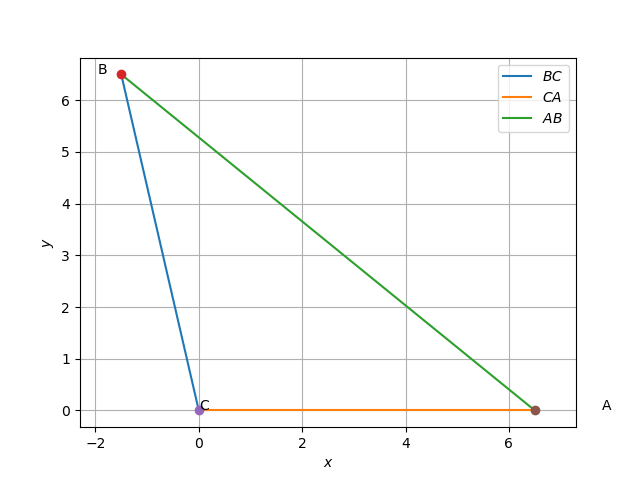
\includegraphics[width=\columnwidth]{diagram-1.png}
\caption{Isosceles  triangle $\triangle OLD$}
\label{fig:isosceles_triangle}	
\end{figure}
\end{document}
